\chapter{Computer Languge}
\label{ch:Computer Languge}

\section{blender}

Open the blender in the terminal as 
\begin{verbatim}
/Applications/blender/blender.app/Contents/MacOS/blender
\end{verbatim}
So the system console works.

\begin{itemize}
\item everytime you move the object, there is a python code appares at the top of the scene, which could be copy into the Scripting.
\item  next
\end{itemize}


\section{OSX}

Find the file location:
\begin{verbatim}
Method 1: From the Terminal, type "open -a Finder /usr/local/bin".

Method 2: From Finder's "Go" menu, select "Go to folder...". That'll bring up a window in which you can type "/usr/local/bin".
\end{verbatim}

\subsection{burn orignal.iso into usb}

in the terminal input those following command:

\begin{itemize}
\item diskutil list
\item diskutil unmountDisk /dev/disk2\footnote{The usb disk}   
\item sudo dd if=orignal.iso\footnote{you can drag the file into here} of=/dev/disk2\footnote{The usb disk} bs=1m
\end{itemize}

Note:
the procession will take 20-30 mins.

\section{python}

Using pypy 
\begin{verbatim}
At the command line, instead of:
python my_program.py

Use:
path/to/where/you/installed/pypy my_program.py
\end{verbatim}

\section{Fortran}

The intriduction

Firstly, you need to know how to run the Fortran independtly, not with communication with python or others. Such as: gfortran name.f90 -llapack -lblas.

The subroutine programe of Fortran could be used to improve the calculation speed of python. There are two ways to do this job.

\begin{itemize}
	\item f2py, which is general way to compile fortran to .os file that could be called in python \url{https://docs.scipy.org/doc/numpy-dev/f2py/}.
	\item jupyter, the previser version is ipyhotn, which give a more easy and simple way to call fortran subroutine in python when subroutine programe is short and without using libs \url{http://nbviewer.jupyter.org/github/mgaitan/fortran_magic/blob/master/documentation.ipynb}.
\end{itemize}

Note: Jupyter is very good and useful tool to develope the programe, because that it could show the calculation result within the code. Moreover, you also could edit the word in bolcks, which is similar with Mathematica files. But, sometimes, I suspect its calculaton result. I feel that I cannot control the memory space. I have tested the case that fortran subroutin contains the lib. Even I delete the lib, it still give the right result. But if I just change to the wrong subroutine name, it does not work. So, I think it does not totally clear the previous memory when you run it second time.  


There are many good subroutine programes we could use, please see the web : \url{https://people.sc.fsu.edu/~jburkardt/index.html}


Run the excutable file
\begin{verbatim}
./a.out
\end{verbatim}


\subsection{Package }

Today, I’ve installed two popular packages \footnote{ \url{http://fortranwiki.org/fortran/show/Libraries}}:

LAPACK, see http://www.netlib.org/lapack/

BLAS, see http://www.netlib.org/blas/

Both packages are required when you deal with linear algebra operations, e.g. solving linear equation systems. Originally, both packages were written in FORTRAN, but I want to use them coding in C++. The solution is to create a libraray! There’re a few steps to consider while installing the packages. First, you have to install BLAS, because LAPACK requires it. If you have downloaded both packages, unzip them. Switch to the BLAS folder and execute
\begin{verbatim}
\$ make
\end{verbatim}
to compile all fortran files. After that, execute

\begin{verbatim}
 \$ mv blas_LINUX.a libblas.a
\end{verbatim}
to rename the created library. Now, you created a library called “libblas.a”. You just copy that file to your library folder. Therefore execute the following command

\begin{verbatim}
 sudo cp libblas.a /usr/local/lib/
\end{verbatim}
Et voila. You’ve installed the BLAS package. 

Now switch to the LAPACK folder and adjust the file “make.inc”. If you set all parameter correctly, execute the command

\begin{verbatim}
sudo cp make.inc.example make.inc
sudo make blaslib
sudo make
\end{verbatim}

\textbf{sudo make blaslib} produces the \textbf{librefblas.a} file, then change the name, and copy it to the /usr/local/lib/.\footnote{All libs shoud be added into \textbf{/usr/local/lib/}, where is the defort location for gfortran libs. In this way, the compile is very esay; \textbf{gfortran name.f90 -llapack -lblas}}

\begin{verbatim}
 sudo cp librefblas.a libblas.a
 sudo cp libblas.a /usr/local/lib/
 sudo cp liblapack.a /usr/local/lib/
\end{verbatim}

In this way, we have put two libs "liblapack.a and libblas.a" into the PATH. Congratulation, you’ve installed BLAS and LAPACK on Mac OS!

Compile the .f90 file:

\textbf{gfortran name.f90 -llapack -lblas}


中文参考 \url{http://www.poluoluo.com/server/200807/19872.html}: 如果编译和测试顺利的话会在源代码的根目录下生成三个文件 liblapack.a、libblas.a、libtmglib.a. liblapack.a 和 libblas.a 就是我们所需要的库函数。它们的使用有两种途径:

a)拷贝liblapack.a 和 libblas.a 到 /usr/local/lib/ 目录下,或者它们所在的目录加入到 /usr/local/lib/环境变量中,或者在编译时候加上 “-L lapack所在目录/” 选项。编译的时候加上编译选项 -llapack -lblas.
 
b) 编译的时候直接把 liblapack.a 和 libblas.a 一起同需要编译的代码一起编译。比如 要编译的文件为 main.f90 编译器为 gfortran.  \textbf{gfortran main.f90 lapack.a blas.a}

GFORTRAN guesses the source code formatting based on the file extension. For .f90 files, it will assume it’s working with FORTRAN 90 source code and use free formatting rules. For .f and .for files, it will assume the file is F77 source code and use fixed formatting rules. I believe this is the problem you’re experiencing. You can override the defaults with -ffixed-form and -ffree-form.

Using \textit{xcode},

\begin{itemize}
\item  choosing "Type" to be "Fortran 90 Source" could make the code color, but not  "Fortran 77 Source" and "Fortran Source"
\item  only one file could exist
\item  only could comple the ".f90" file 

\end{itemize}

\subsection{Modern Fortran Explained}

the Fortran 90 standard was much more a development of the language, introducing features which were new to Fortran, but were based on experience in other languages. The main features of Fortran 90 were, first and foremost, the array language and abstract data types. Last but not least were the new free source form, an improved style of attribute-oriented specifications, the implicit none statement, and a mechanism for identifying redundant features for subsequent removal from he language.

One list contains the deleted features, those that have been removed. Since Fortran 90 contained the whole of Fortran 77, this list was empty for Fortran 90 but was not for Fortran 95. The obsolescent features that were deleted from Fortran 95 are still being supported by most compilers, because of the demand for old tried and tested programs to continue to work. Thus, the concept of obsolescence is really not working as intended, but at least it gives a clear signal that certain features are outmoded, and should be avoided in new programs and not be taught to new programmers.

A drawback of the Fortran 77 standard was that it made no statement about requiring processors to provide a means to detect any departure from the allowed syntax by a program, as long as that departure did not conflict with the syntax rules defined by the standard. The new standards are written in a different style from the old one. The syntax rules are expressed in a form of BNF with associated constraints, and the semantics are described by the text.

Any Fortran statement (that is not part of a compound statement) may be labelled, in order to be able to identify it. For some statements a label is mandatory. A statement label precedes the statement, and is regarded as a token. The label consists of from one to five digits, one of which must be nonzero. An example of a labelled statement is

100 continue

Leading zeros are not significant in distinguishing between labels. For example, 10 and 010 are equivalent.

\begin{verbatim}
selected_int_kind(6) 
\end{verbatim}
is an intrinsic inquiry function call, and it returns a kind parameter value that yields the range \textbf{−999999 to 999999} with the least margin

The default kind consists of a string of characters enclosed in a pair of either apostrophes or quotation marks. 

If expr is not of the same type or kind as variable, it will be converted to that type and kind before the assignment is carried out.

$i <0$ integer relational expression

In this case, and whenever either or both of the two components consist of numeric expressions, the rules state that the components are to be evaluated separately, and converted to the type and kind of their sum before the comparison is made.

\begin{verbatim}
character(len=5) :: fill
 fill(1:4) = ’AB’
\end{verbatim}
$fill(1:4)$ will have the value ABbb (where b stands for a blank character). The value of $fill(5:5)$ remains undefined, that is, it contains no specific value and should not be used in an expression. As a consequence, fill is also undefined.

The most important form is that of a block construct, that is a construct which begins with an initial keyword statement, may have intermediate keyword statements, and ends with a matching terminal statement, and that may be entered only at the initial statement. 

\begin{verbatim}
[name:] do
\end{verbatim}
In practice, a means to exit from an endless loop is required, and this is provided in the form of the exit statement:

\begin{verbatim}
exit [name]
\end{verbatim}

where name is optional and is used to specify from which do construct the exit should be taken in the case of nested constructs.

\begin{verbatim}
cycle [name]
\end{verbatim}

which transfers control to the end do statement of the corresponding construct.

A complete program must, as a minimum, include one \textbf{main program}. This may contain statements of the kinds that we have met so far in examples, but normally its most important statements are invocations or calls to subsidiary programs known as subprograms. A subprogram defines a \textbf{function} or a \textbf{subroutine}. 

Another way to stop program execution is to execute a \textbf{stop} statement. This statement may appear in the main program or any subprogram. A well-designed program normally returns control to the main program for program termination, so the \textbf{stop} statement should appear there. However, in applications where several \textbf{stop} statements appear in various places in a complete program, it is possible to distinguish which of the \textbf{stop} statements has caused the termination by adding to each one a stop code consisting of a default character constant or a string of up to five digits whose leading zeros are not significant.
\begin{verbatim}
   stop
   stop ’Incomplete data. Program terminated.’
   stop 12345
\end{verbatim}

\section{linux}

pwd, print working directory, which outputs (displays) the current directory.\\
cd,  change your current direc- tory (see above) will change the prompt but will not display any output. \\
mkdir, Make a new directory\\
touch, Make a new empty file\\
cp, Copy a file\\
mv, Move a file\\
rm, Remove a file or directory (learn about the -r option)\\
less, Show the contents of a file in a scrolling buffer\\
\vspace{5mm}
Fortunately, most commands have a manual. To read, use the man command. Pass the name of the command you want to learn about as it’s only argument. For instance to learn more about ls, run\\
man ls


\section{C++}

As with all formatting manipulators, you must include the header file iomanip to use setprecision. 

- You can control the number of significant digits with which floating-point values are displayed by using the setprecision manipulator. 
The number inside the parentheses after the word setw specifies the field width for the value immediately following it. 
\begin{verbatim}
* cout << setprecision(2) << fixed; 
\end{verbatim}

- When the fixed manipulator is used, all floating point numbers that are subsequently printed will be displayed in fixed point notation, with the number of digits to the right of the decimal point specified by the setprecision manipulator. 

- When the fixed and setprecision manipulators are used together, the value speci- fied by the setprecision manipulator will be the number of digits to appear after the decimal point, not the number of significant digits. 

\begin{verbatim}
* // Display the sales figures. 
* 23  cout << "\nSales Figures\n"; 
* 24  cout << "-------------\n"; 
* 25  cout << setprecision(2) << fixed; 
* 26  cout << "Day 1: " << setw(8) << day1 << endl; 
* 27  cout << "Day 2: " << setw(8) << day2 << endl; 
* 28  cout << "Day 3: " << setw(8) << day3 << endl; 
* 29  cout << "Total: " << setw(8) << total << endl; 
* 30  return 0; 

\end{verbatim}

Pointers 


- 9.1 Getting the Address of a Variable

Getting the address of a variable is accomplished with an operator in C++. When the address operator ($\&$) is placed in front of a variable name, it returns the address of that variable. Here is an expression that returns the address of the variable amount: 

\begin{verbatim}
* & amount 
And here is a statement that displays the variable’s address on the screen: 
* cout << & amount; 
\end{verbatim}



\chapter{Latex}

\section{ MacTeX 配置中文支持}

目前来说,结合 xeCJK 宏包使用 XeLaTeX 编译,应该是最方便的方式了。 XeLaTeX 要求 .tex 文档保存为 UTF-8 编码。所以要做的事情只有两件 \footnote{http://liam0205.me/2014/11/02/latex-mactex-chinese-support/}:

\begin{enumerate}
	\item 配置一个 UTF-8 的编辑环境;
    \item 用 xeCJK 的语法选择合适的字体。
\end{enumerate}

XeTeX 在 Mac OS X 下的行为和 Windows/Linux 下不大一样。Mac 底下,XeTeX 并不使用 fontconfig 库来搜索字体,所以我们没法在终端里通过 fc-list 命令来查看可用的字体列表。不过 Mac 里提供了名为「字体册」的程序,来列出系统中所有可用的字体信息。

其实这样的设计挺讨厌的,TeX Live 自带了许多开源字体,因此没有办法很好地使用。必须用字体名而不是字族名来调用这些字体,实在是不太方便。当然,如果有需要,我们可以把 TeX 里自带的这些开源字体用硬链接的方式,添加到 Mac 的字体目录下。

打开字体册程序,找到需要的字体信息:

\begin{figure*}
	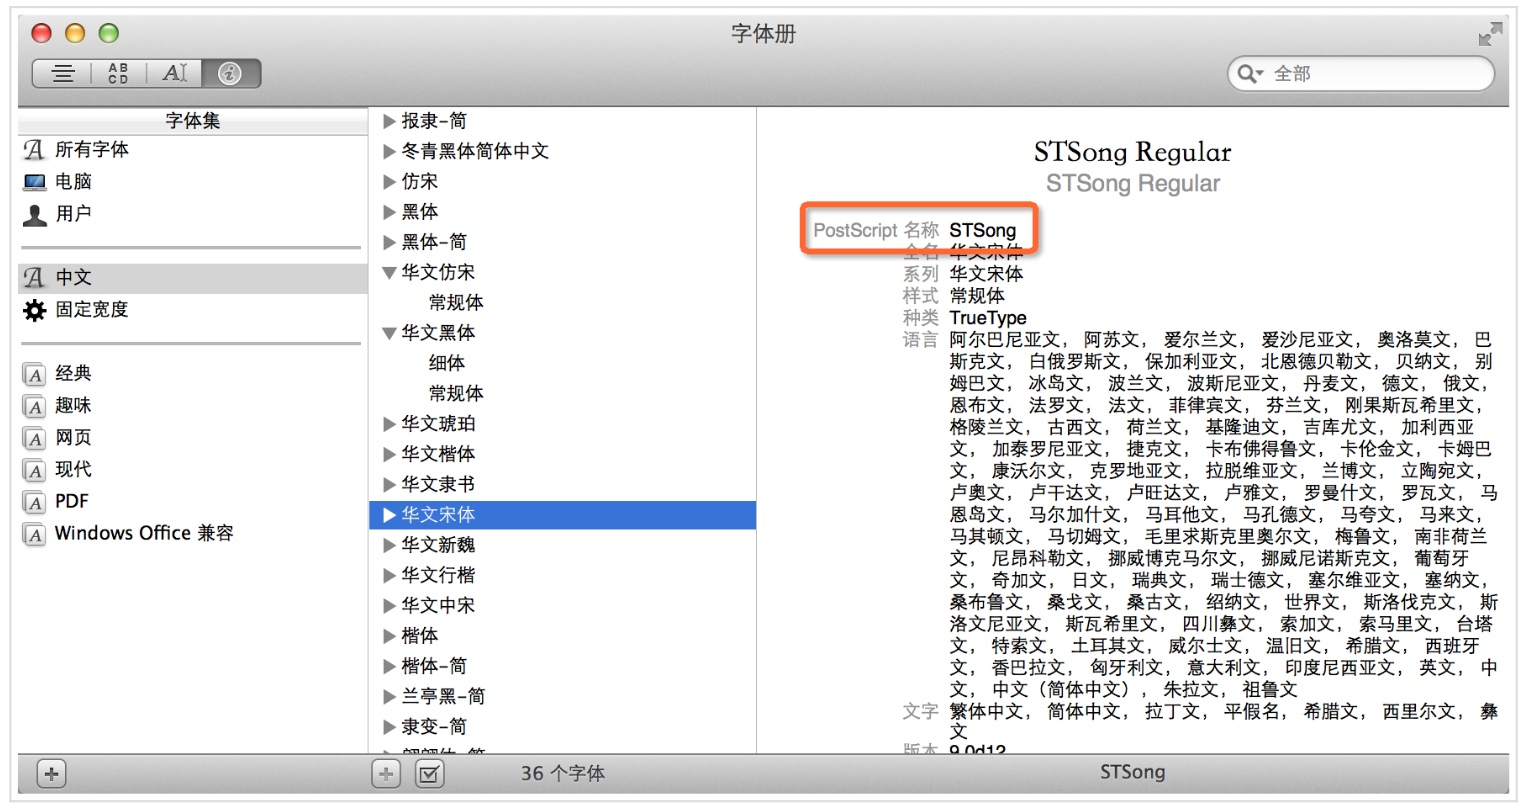
\includegraphics{chapter/CL_fig/mac字体}
	\caption{mac字体}
\end{figure*}

这里的 PostScript 名称就是我们需要的信息,我们记下华文宋体的名字:「\colorbox{red}{STSong}」。你还可以按需找到其他字体的名字,比如华文中宋、华文楷体、华文黑体等字体的名字。

Note: \colorbox{red}{在mac里面不是SimSun字体,而是STSong}, 在win下面是STSong。


\section{texmaker}

\subsection{short cut}

see the \textbf{texmaker $\rightarrow$ preference $\rightarrow$ Shortcut}

\section{compile latex using terminal}

latexmk -xelatex filename\footnote{1. you should cd to the filename dic. 2.the compile speed is faster, I think, using this way.}

You need to compile the file two times to generate the table of content/figures/tables lists. 

\section{Latex + sublime}

package "Latexing" is for color display.

\begin{verbatim} 
%!TEX program = xelatex  
\end{verbatim} \sidenote{determine the engine: xelatex}


\begin{verbatim}
\usepackage{fontspec, xunicode, xltxtra}  
\setmainfont{Hiragino Sans GB}  

or using 

\usepackage{xeCJK}
\setCJKmainfont{SimSun}

\end{verbatim} \sidenote{chinese words}

\begin{verbatim}
\usepackage{xcolor}
\usepackage{hyperref}
  \hypersetup{pagebackref,
              backref,
              colorlinks,
              linkcolor=blue,
              anchorcolor=red,
              citecolor=blue,
              urlcolor=magenta} 
\end{verbatim} \sidenote{hyperlink setup}
                 
\begin{verbatim}                 
\usepackage{geometry}
\newgeometry{left=1in,
             right=1in,
             top=1in,
             bottom=1in,
             headsep=1cm,
             marginparwidth=85pt,
             marginparsep=11pt}             
\end{verbatim} \sidenote{Page Layout}

\begin{figure*}
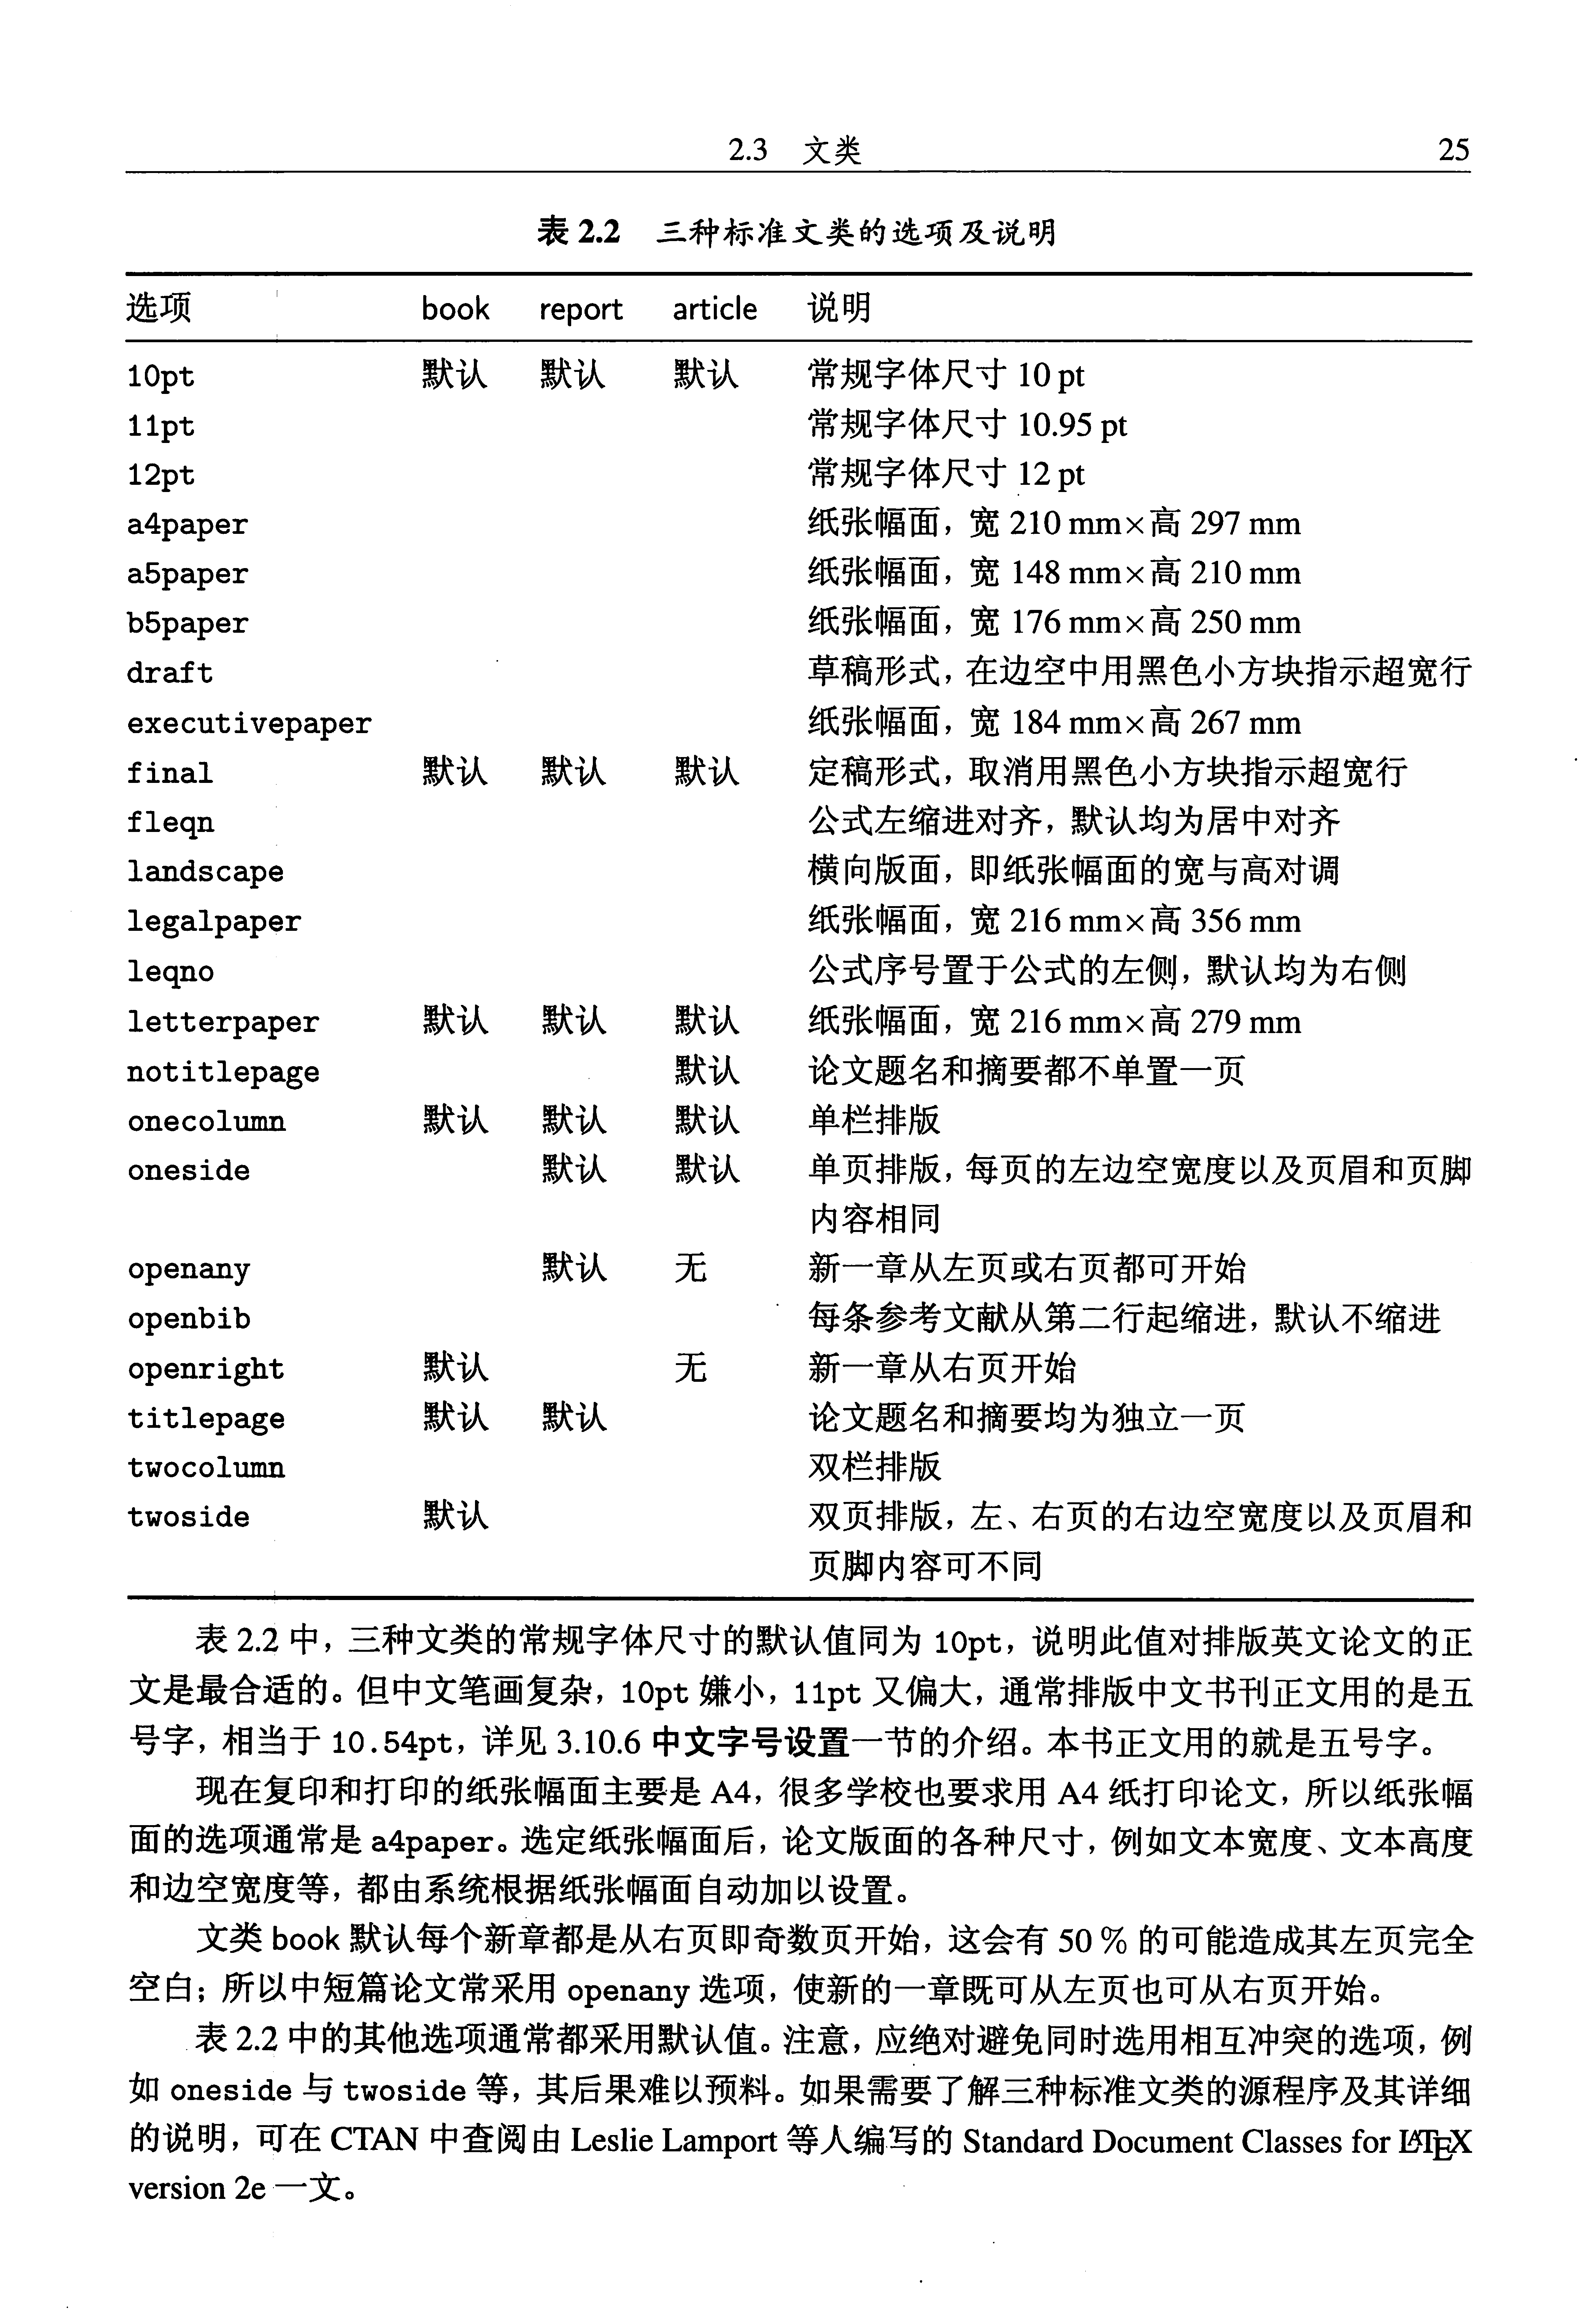
\includegraphics{figures/文类.jpg}
      \caption{文类}
\end{figure*}

\begin{figure*}
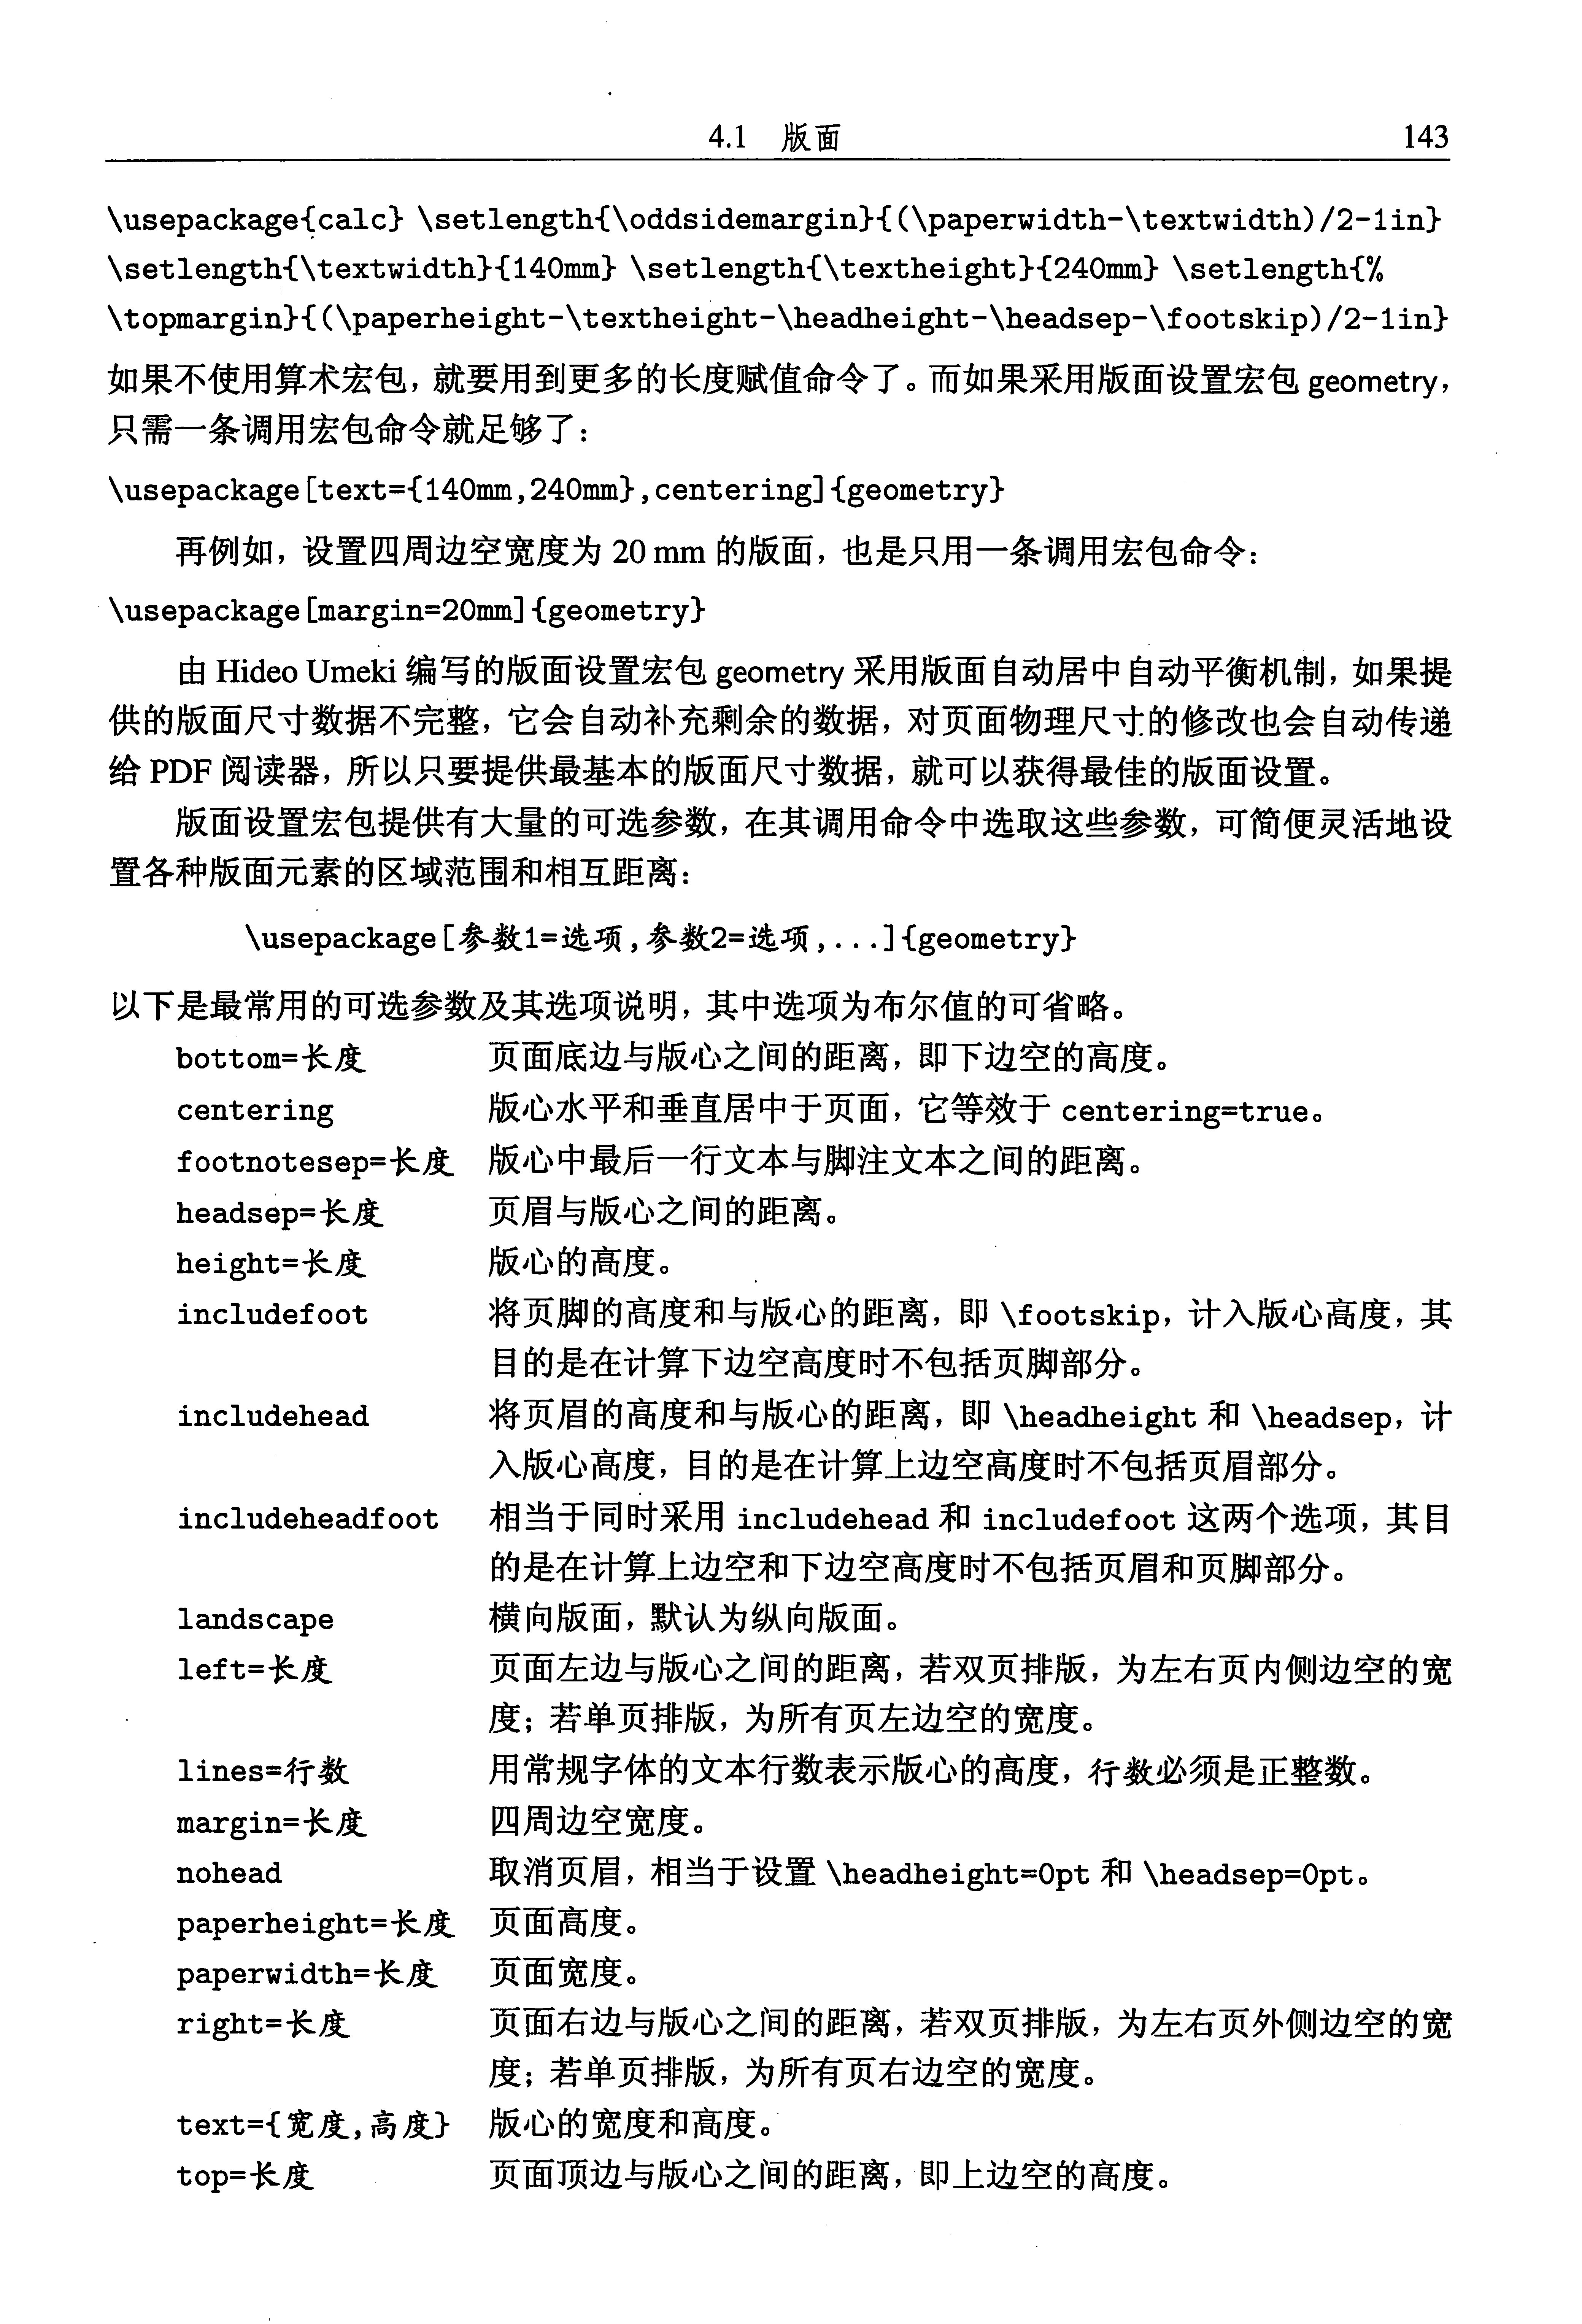
\includegraphics{figures/版面.jpg}
      \caption{版面}
\end{figure*}

\begin{figure*}
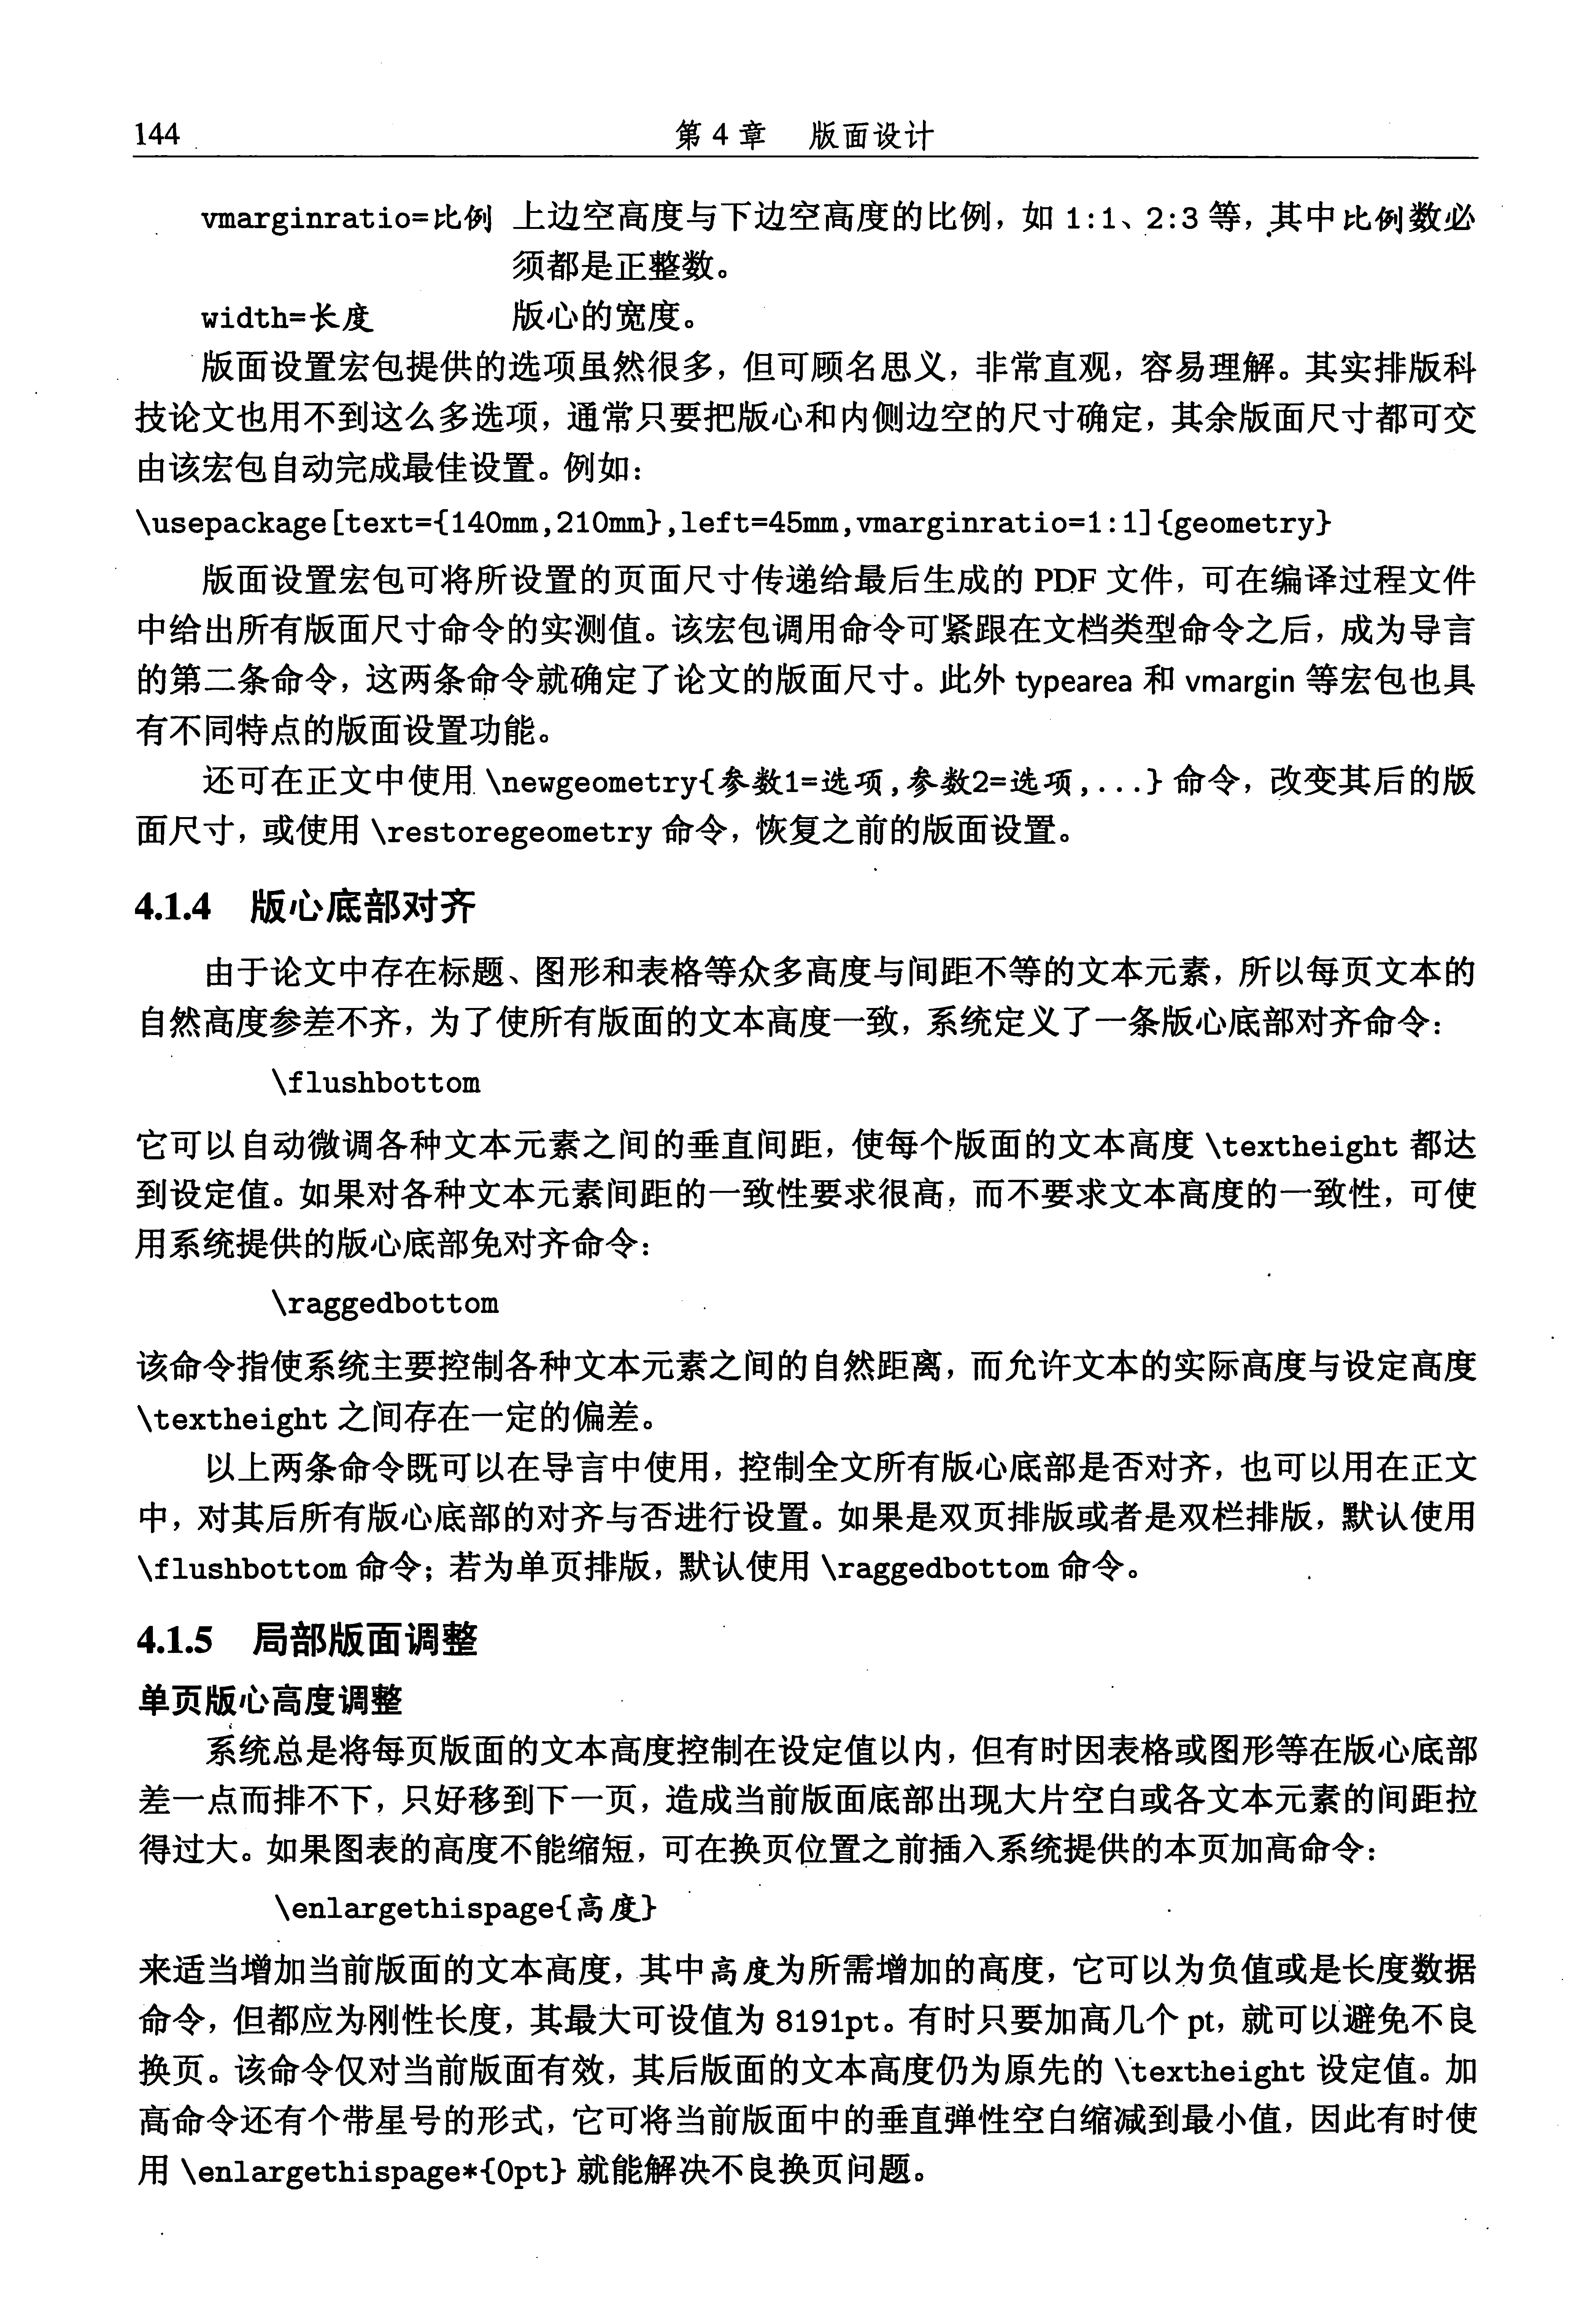
\includegraphics{figures/版面设计.jpg}
      \caption{版面设计}
\end{figure*}

\begin{figure*}
	 includegraphics{figures/字体设计.jpg} 
	 caption{字体设计} 
\end{figure*}


\chapter{Lyx}

\subsection{Setting up LyX to work with XeTeX}

\begin{itemize}
\item check in the menu \textcolor{red}{Document $>$ Settings$>$ Fonts} the option \textcolor{red}{Use non-TeX fonts (via XeTeX/LuaTeX)}. Then you can immediately use the menu \textcolor{red}{View $>$ PDF (XeTeX)}.
\item  Using OpenType fonts (otf) in XeTeX math mode (LyX 2.1)...
\end{itemize}

\paragraph{Setting up XeTeX for CJK scripts}

If you follow the instructions below you can just go ahead and use CJK characters like 猫 into your document (this one means 'cat'). Only CJK characters will use a CJK font and everything else will remain untouched.
Download the xeCJK package from \url{http://www.ctan.org/login/auth}, if it is not yet installed (it should be included in TeXLive and MikTeX).
Add the following lines to Document \textrightarrow Settings \textrightarrow LaTeX Preamble:

\begin{verbatim}
\usepackage{xeCJK}
\setCJKmainfont{Sazanami Mincho}
\end{verbatim}


The detail please see web \url{https://wiki.lyx.org/LyX/XeTeX}

\subsection{LyX + LaTeX}

有些时候Lyx Export的Latex代码不可以直接被Latex编译;同样在Lyx使用Latex代码也会出错,如"input{**.tex}"。为此可以采用如下方法\footnote{1.Lyx使用的是同样的模板;2.Latex的main.tex文件可能需要加载package}:

\begin{itemize}
  \item 在Lyx中写好内容,然后Export Xelatex文件 "name.tex"
  \item 打开“name.tex”文件,删除开头和结尾,只保留主题内容
  \item 此时的”name.tex“ 文件可以被Latex 和 Lyx调用
\end{itemize}


\subsection{input “nameoflayout.layput” into the lyx  and “nameofclass.cls” into latex}

input “nameofclass.cls” into latex\\
Find the location of class
- sudo find / -name revtex4\\
/usr/local/texlive/2016/texmf-dist/tex/latex/

- sudo mv iopart /usr/local/texlive/2016/texmf-dist/tex/latex/

- sudo mktexlsr

input “nameoflayout.layout” into lyx\\
Find the location of layout\\
- sudo find / -name layouts\\
- /Applications/LyX.app/Contents/Resources/layouts\\
\vspace{5mm}

For LyX to see and use the new files, you will need to run Tools > Reconfigure.
Go to Document > Settings > Document Class.  Then from the drop down menu, select “name”.\\
\vspace{5mm}

Note:
\begin{itemize}
  \item There are three file names: nameofclass, nameoflayout and nameforducumentsetting
  \item \textbackslash DeclareLaTeXClass[“nameofclass”]{“namefordocumentsettting”}
  \item In this example, namefordocumentsettting is the name of the LaTeX document class (nameoflcass.cls) and the information in curly brackets is a description which will make it easier to find in the LyX document settings pane.
\end{itemize}

useful web: \url{http://www.oak-tree.us/blog/index.php/2009/11/02/custom-lyx-nih}






Preprocessor directives, like $\#$include statements, simply end at the end of the line and never require semicolons. The beginning of a function, like int main(), is not a complete statement, so you don’t place a semicolon there either. 


% Preview source code for paragraph 0

int main() This marks the beginning of a function. A function can
be thought of as a group of one or more programming statements that
collectively has a name. The name of this function is main, and the
set of parentheses that follows the name indicate that it is a function.
The word int stands for \textquotedblleft integer.\textquotedblright{}
It indicates that the function sends an integer value back to the
operating system when it is finished executing. 

% Preview source code for paragraph 0

\chapter{Tools}
\section{sublime}

set the package $sublime tex \rightarrow preferences \rightarrow package setting$

Sublime Text 使用技巧
。

Sublime快捷键 : \url{https://www.zhihu.com/question/24896283?rf=19976788}

\begin{verbatim}

备注:具体符号对应的按键

⌘Command key
⌃Control key
⌥Option key
⇧Shift Key
为了方便大家记忆,将快捷键分成了8个类型, 分别为

Edit(编辑)
Selection(光标选中)
Find(查找)
View(视图)
Go to(跳转)
Project(工程)
General(通用)
Tabs(标签)
_______________________________________________________
Edit(编辑)
command + [ : 向左缩进 | Left indent
command + ] : 向右缩进 | Right Indent
command + control + ↑ : 与上一行互换(超实用!)| Swap line up
command + control + ↓ : 与下一行互换(超实用!)| Swap line down
command + ← : 去往行的开头 | Beginning of line
command + → : 去往行末尾 | End of line
________________________________________________________
Selection(光标选中)
command + D : 选中相同的词 | Expand selection to words
command + control + G : 多重文本光标选中(再也不用⌘ D一个一个的找啦)| Expand all selection to words
________________________________________
Go to(跳转/定位)
command + P : 跳转文件(很方便)| Go to anything
___________________________________________
Project(工程)
command + control + P : 在保存过的工程中切换,随意变换工程环境|Switch project window

__________________________________________
General(通用)
command + shift + P 打开命令行| Command prompt


\end{verbatim}




\section{git and github}\footnote{\url{https://git-scm.com/book/zh/v2/Git-基础-远程仓库的使用}}

\begin{verbatim}

$ git init
该命令将创建一个名为 .git 的子目录,这个子目录含有你初始化的 
Git 仓库中所有的必须文件,这些文件是 Git 仓库的骨干。

$ git add *.c
$ git add LICENSE
$ git commit -m 'initial project version'

克隆现有的仓库:
$ git clone https://github.com/schacon/ticgit

查看已暂存和未暂存的修改
如果 git status 命令的输出对于你来说过于模糊,你想知道具体修改了什么地方,
可以用 git diff 命令。此命令比较的是工作目录中当前文件和暂存区域快照之间的差异,
 也就是修改之后还没有暂存起来的变化内容。若要查看已暂存的将要添加到下次
 提交里的内容,可以用 git diff --cached 命令。(
 Git 1.6.1 及更高版本还允许使用 git diff --staged,效果是相同的,但更好记些。)

$ git diff --staged
diff --git a/README b/README
new file mode 100644
index 0000000..03902a1
--- /dev/null
+++ b/README
@@ -0,0 +1 @@
+My Project

提交更新
现在的暂存区域已经准备妥当可以提交了。 在此之前,请一定要确认还有什么修改过的
或新建的文件还没有 git add 过,否则提交的时候不会记录这些还没暂存起来的变化。 
这些修改过的文件只保留在本地磁盘。 所以,每次准备提交前,先用 git status 看下,
是不是都已暂存起来了, 然后再运行提交命令 git commit:


移除文件
要从 Git 中移除某个文件,就必须要从已跟踪文件清单中移除(确切地说,是从暂存区域移除)
,然后提交。 可以用 git rm 命令完成此项工作,并连带从工作目录中删除指定的文件,
这样以后就不会出现在未跟踪文件清单中了。

另外一种情况是,我们想把文件从 Git 仓库中删除(亦即从暂存区域移除),但仍然希望保留
在当前工作目录中。 换句话说,你想让文件保留在磁盘,但是并不想让 Git 继续跟踪。 当你
忘记添加 .gitignore 文件,不小心把一个很大的日志文件或一堆 .a 这样的编译生成文件添加
到暂存区时,这一做法尤其有用。 为达到这一目的,使用 --cached 选项:

$ git rm --cached README
git rm 命令后面可以列出文件或者目录的名字,也可以使用 glob 模式。 比方说:

$ git rm log/\*.log
注意到星号 * 之前的反斜杠 \, 因为 Git 有它自己的文件模式扩展匹配方式,所以我们不用 
shell 来帮忙展开。 此命令删除 log/ 目录下扩展名为 .log 的所有文件。 类似的比如:

$ git rm \*~
该命令为删除以 ~ 结尾的所有文件。



$ git remote -v
origin	https://github.com/schacon/ticgit (fetch)
origin	https://github.com/schacon/ticgit (push)

$ git remote add pb https://github.com/paulboone/ticgit
$ git remote -v
origin	https://github.com/schacon/ticgit (fetch)
origin	https://github.com/schacon/ticgit (push)
pb	https://github.com/paulboone/ticgit (fetch)
pb	https://github.com/paulboone/ticgit (push)

现在你可以在命令行中使用字符串 pb 来代替整个 URL。
 例如,如果你想拉取 Paul 的仓库中有但你没有的信息,可以运行 git fetch pb:

$ git fetch pb

推送到远程仓库
当你想分享你的项目时,必须将其推送到上游。 这个命令很简单:
git push [remote-name] [branch-name]。 当你想要将 master 分支推送到 origin 服务器时
(再次说明,克隆时通常会自动帮你设置好那两个名字),那么运行这个命令就可以将你所做的备份到服务器:

$ git push origin master

\end{verbatim}








